\section{Process Perspective}
hallo \cite{devopshandbook}
\subsection{Monitoring and logging}
For monitoring we use Grafana. Our board shows requests duration, errors rate, top 10 unhandled exception endpoints and more (for visualization of the board, see appendix \ref{appendix:grafana}). We have used the board to get an overview of where to put our focus, ie. which endpoints to improve, which errors to fix, etc. Moreover, we have gained insights into the health of the system and gotten an impression of how the backend and frontend handle the requests.

For logging, we use Grafana and Loki. It seemed obvious to continue our work with Grafana in order to keep the system setup as simple as possible. The logs are divided into Information, Warning, Debug and Error. All logging statements are placed in the controllers, such that we have information about the users' whereabouts in the system. For example, we log when a user logins whether successful or unsuccessful.
\subsection{Security Assessment}
Based on our security assessment, which can be found in appendix C, we constructed the following risk matrix:
\begin{figure}[H]
    \centering
    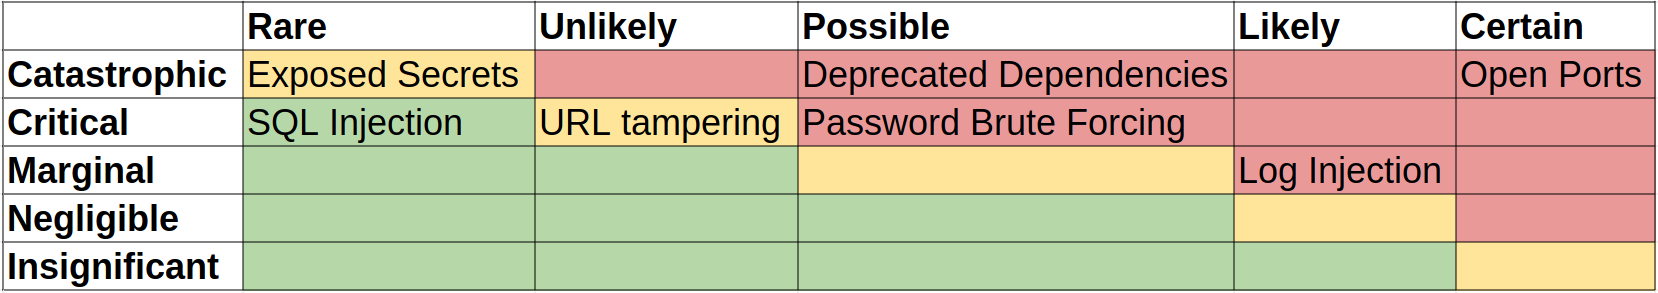
\includegraphics[width=0.7\linewidth]{images/risk-matrix.png}
    \caption{Risk matrix from security assessment}
    \label{fig:enter-label}
\end{figure}
We decided to focus on the scenarios in the red zone, as they would be the cause of most damage. Due to the group not having enough knowledge about how the simulator worked in regards to creating users and logging in, we didn't move further with the \textit{Password Brute Forcing} scenario, whereas the solution would have been to incorporate 2FA, password requirements and time-out limitation for an actual system in production.

For \textit{Log Injection}, we made sure to sanitize user inputs, as they beforehand were put directly into the log, which could be exploited to hide ill-intentioned actions. We thereby hardened the system against injection attacks.
With \textit{Depricated Dependencies}, we chose to integrate the tool \textit{dependabot} into our CI/CD pipeline to watch out for outdated dependencies. This helps us ensure that an adversary isn't able to take advantage of the team not being aware of vulnerabilities in variuos of the used tools.

\textit{Open Ports} was deemed the biggest risk, as this was most likely the reason for us being hacked, which we have written more about in our lesson about being hacked. We used the tool \textit{nmap} to check for open ports, where we then tried to close the open port used for Prometheus. It was unclear if we were successful as \textit{nmap} kept showing the port as open despite seeing the firewall configuration saying otherwise on the server itself.
We also attempted to switch from HTTP to HTTPS, as it would strengthen the overall security of our application, but here we ran into several bureaucratic issues with changing the name servers for the domain, which resulted in us running out of time of the task. Ideally, this would have been accomplished to further harden our system's security.
